\chapter{Détection des scans réseau et corrélation des événements}

\section{Introduction}

Après la mise en place du mécanisme de détection des attaques SSH, de la notification automatique via Telegram et du blocage dynamique des adresses IP sur le routeur Cisco, la cinquième phase du projet ANSDS vise à améliorer la capacité de détection du système.

La stratégie initiale reposait principalement sur l'observation des paquets TCP SYN destinés au port SSH. Cette approche permet de détecter rapidement des tentatives de connexion, mais un paquet SYN isolé ne constitue pas nécessairement une activité malveillante. Une connexion SSH légitime commence également par l'émission d'un paquet TCP SYN.

La Phase 5 introduit donc une deuxième catégorie d'activité suspecte : les scans réseau réalisés avec Nmap. L'objectif est de détecter une activité de reconnaissance pouvant précéder une tentative d'intrusion.

Les scans étudiés durant cette phase sont :

\begin{itemize}

\item TCP SYN Scan (\texttt{-sS}) ;

\item TCP FIN Scan (\texttt{-sF}) ;

\item TCP NULL Scan (\texttt{-sN}) ;

\item TCP Xmas Scan (\texttt{-sX}).

\end{itemize}

La Phase 5 conserve l'architecture modulaire développée lors des phases précédentes et repose sur Scapy pour l'analyse du trafic \cite{scapy_docs}, Python pour la logique de détection, Telegram pour les notifications, Netmiko pour l'automatisation Cisco et les ACL Cisco IOS pour le blocage réseau \cite{netmiko_docs,cisco_ios}. Cette architecture correspond à l'évolution prévue du système vers une détection multi-indicateurs.

\section{Objectifs de la phase}

Les objectifs principaux de cette phase sont les suivants :

\begin{itemize}

\item détecter les comportements caractéristiques des scans Nmap ;

\item prendre en charge plusieurs types de scans TCP ;

\item identifier l'adresse IP source du scan ;

\item identifier l'adresse IP destination ;

\item analyser les drapeaux TCP observés ;

\item mesurer le nombre de ports distincts ciblés ;

\item utiliser une fenêtre temporelle afin d'identifier un comportement de reconnaissance ;

\item réduire les faux positifs liés aux paquets TCP isolés ;

\item corréler une activité de scan avec des événements SSH ;

\item transmettre une alerte de sécurité via Telegram lorsqu'une activité suspecte est confirmée ;

\item appliquer automatiquement un blocage temporaire sur le routeur Cisco ;

\item journaliser les événements importants du système ;

\item supprimer automatiquement le blocage après expiration de la durée configurée.

\end{itemize}

La conception de la Phase 5 suit une approche progressive afin de conserver la modularité des composants existants et d'éviter de rendre le moteur de détection SSH inutilement complexe.

\section{Évolution de la stratégie de détection}

\subsection{Limites de la détection SSH initiale}

Lors des phases précédentes, le moteur de détection surveillait les paquets TCP SYN destinés au port 22.

Cette méthode présente un avantage important : elle permet d'identifier une tentative de connexion dès le début de l'établissement de la connexion TCP.

Cependant, un paquet SYN isolé peut également correspondre à une activité parfaitement légitime.

La détection doit donc prendre en compte le comportement global de la source plutôt qu'un paquet unique.

\subsection{Introduction de la détection Nmap}

La Phase 5 étend le moteur afin d'identifier les comportements associés aux scans Nmap.

Un scan réseau se caractérise notamment par l'envoi rapide de paquets vers plusieurs ports de destination.

Le détecteur analyse donc plusieurs informations :

\begin{itemize}

\item l'adresse IP source ;

\item l'adresse IP destination ;

\item les drapeaux TCP ;

\item les ports de destination ;

\item le nombre de ports distincts ;

\item la fenêtre temporelle.

\end{itemize}

Le principe général retenu est le suivant :

\begin{center}

Même source IP

$\downarrow$

Même signature TCP

$\downarrow$

Plusieurs ports distincts

$\downarrow$

Courte fenêtre temporelle

$\downarrow$

Événement de scan

\end{center}

Cette approche permet d'éviter de considérer un paquet TCP isolé comme un scan.

\section{Signatures TCP des scans Nmap}

Les différents types de scans étudiés utilisent des combinaisons différentes de drapeaux TCP \cite{scapy_docs}.

\subsection{TCP SYN Scan}

Le SYN Scan est réalisé avec l'option :

\begin{verbatim}

nmap -sS

\end{verbatim}

Les paquets observés contiennent principalement le drapeau TCP :

\begin{verbatim}

SYN

\end{verbatim}

Le détecteur associe ces paquets à l'adresse IP source et aux ports de destination observés.

\begin{figure}[H]

    \centering

    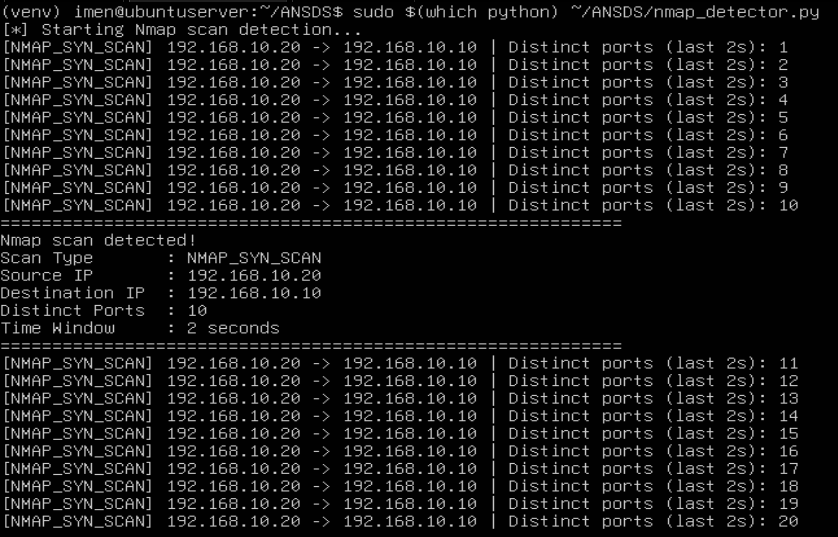
\includegraphics[width=0.95\textwidth]{figures/Fig-05-01_Nmap_SYN_Scan_Detection.png}

    \caption{Détection d'un scan Nmap SYN}

    \label{fig:phase5-nmap-syn}

\end{figure}

\subsection{TCP FIN Scan}

Le FIN Scan est réalisé avec :

\begin{verbatim}

nmap -sF

\end{verbatim}

La signature observée correspond à un paquet TCP contenant le drapeau :

\begin{verbatim}

FIN

\end{verbatim}

Le détecteur identifie cette signature puis vérifie si elle est répétée vers plusieurs ports dans une courte période.

\begin{figure}[H]

    \centering

    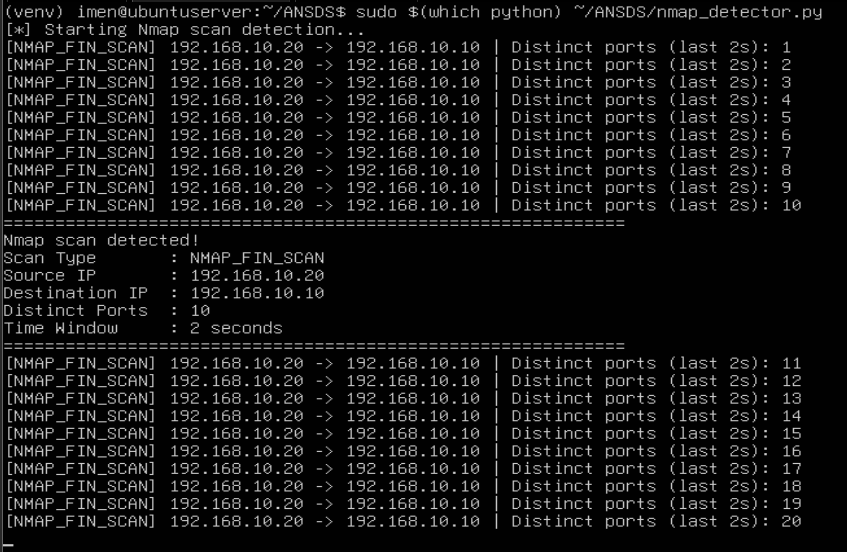
\includegraphics[width=0.95\textwidth]{figures/Fig-05-02_Nmap_FIN_Scan_Detection.png}

    \caption{Détection d'un scan Nmap FIN}

    \label{fig:phase5-nmap-fin}

\end{figure}

\subsection{TCP NULL Scan}

Le NULL Scan est réalisé avec :

\begin{verbatim}

nmap -sN

\end{verbatim}

Dans ce cas, aucun des principaux drapeaux TCP observés dans les autres signatures n'est activé.

La signature considérée par le détecteur correspond donc à l'absence de drapeaux TCP.

\begin{figure}[H]

    \centering

    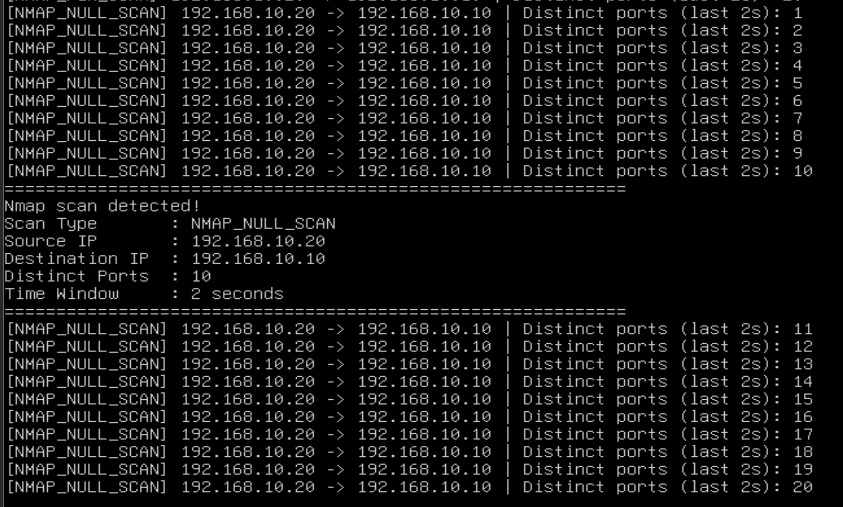
\includegraphics[width=0.95\textwidth]{figures/Fig-05-03_Nmap_NULL_Scan_Detection.png}

    \caption{Détection d'un scan Nmap NULL}

    \label{fig:phase5-nmap-null}

\end{figure}

\subsection{TCP Xmas Scan}

Le Xmas Scan est réalisé avec :

\begin{verbatim}

nmap -sX

\end{verbatim}

La signature observée correspond à la combinaison de plusieurs drapeaux TCP :

\begin{verbatim}

FIN + PSH + URG

\end{verbatim}

Cette combinaison permet au détecteur de distinguer ce comportement des autres signatures étudiées.

\begin{figure}[H]

    \centering

    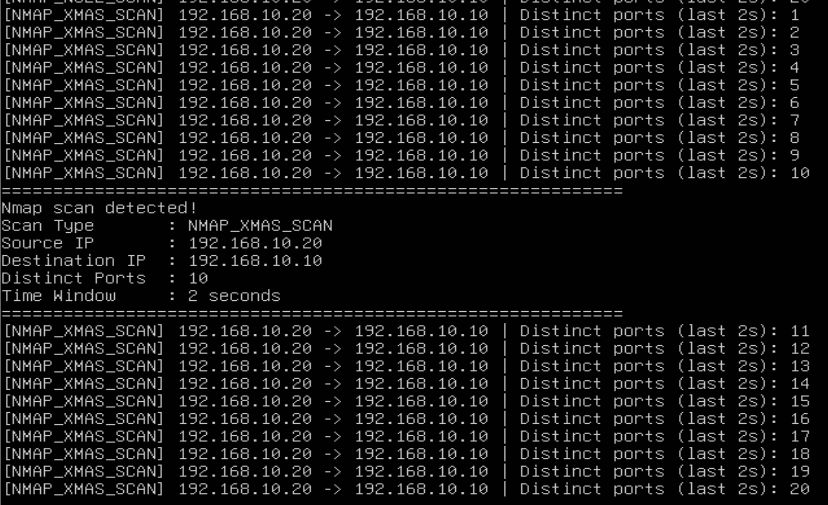
\includegraphics[width=0.95\textwidth]{figures/Fig-05-04_Nmap_XMAS_Scan_Detection.png}

    \caption{Détection d'un scan Nmap Xmas}

    \label{fig:phase5-nmap-xmas}

\end{figure}

\section{Détection comportementale des scans}

La détection ne repose pas uniquement sur la présence d'une signature TCP.

Un paquet isolé peut correspondre à un comportement légitime ou à une communication réseau normale. Pour cette raison, le détecteur conserve les informations relatives aux paquets observés et analyse leur comportement dans une fenêtre temporelle limitée.

Pour une même adresse IP source, le système regroupe les paquets présentant une signature similaire et enregistre les ports de destination ciblés.

Lorsque plusieurs ports distincts sont observés sur une courte période, le comportement devient compatible avec une activité de reconnaissance.

Le mécanisme peut être représenté comme suit :

\begin{center}

Source IP

$\downarrow$

Signature TCP

$\downarrow$

Ports de destination

$\downarrow$

Nombre de ports distincts

$\downarrow$

Fenêtre temporelle

$\downarrow$

Détection Nmap

\end{center}

Cette logique permet de différencier une activité de scan d'un paquet TCP isolé.

\section{Réduction des faux positifs}

La réduction des faux positifs constitue un objectif important de cette phase.

Un système de détection réseau ne doit pas générer une alerte simplement parce qu'un paquet possède une signature particulière.

Un trafic légitime peut contenir des paquets TCP présentant des caractéristiques similaires à celles utilisées par un détecteur.

Le système considère donc plusieurs éléments simultanément :

\begin{itemize}

\item la source du trafic ;

\item la signature TCP ;

\item le nombre de ports ciblés ;

\item la rapidité des requêtes ;

\item la présence éventuelle d'une activité SSH associée.

\end{itemize}

\subsection{Validation du trafic légitime}

Un scénario de trafic légitime a été utilisé afin de vérifier que le détecteur ne considère pas automatiquement toute activité TCP comme un scan Nmap.

La capture suivante présente le trafic utilisé durant cette validation.

\begin{figure}[H]

    \centering

    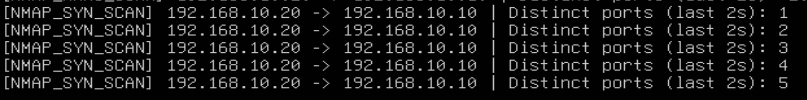
\includegraphics[width=0.95\textwidth]{figures/Fig-05-05_Nmap_Legitimate_Traffic.png}

    \caption{Trafic réseau légitime observé durant la validation}

    \label{fig:phase5-legitimate-traffic}

\end{figure}

Cette validation permet de vérifier que la décision de détection repose sur le comportement global observé plutôt que sur un paquet isolé.

\section{Corrélation avec l'activité SSH}

La détection d'un scan Nmap constitue un indicateur de reconnaissance, mais elle ne permet pas à elle seule de conclure qu'une tentative d'intrusion SSH est en cours.

La Phase 5 introduit donc une logique de corrélation entre l'activité de reconnaissance et l'activité SSH.

Le principe est le suivant :

\begin{center}

Nmap Scan détecté

$\downarrow$

Surveillance de l'activité SSH

$\downarrow$

Évidence d'authentification échouée

$\downarrow$

Corrélation confirmée

$\downarrow$

Événement de sécurité

\end{center}

Cette approche permet de renforcer la décision de sécurité en combinant plusieurs indicateurs plutôt qu'en utilisant une seule observation réseau.

La corrélation entre le scan et l'activité SSH a été validée expérimentalement.

\begin{figure}[H]

    \centering

    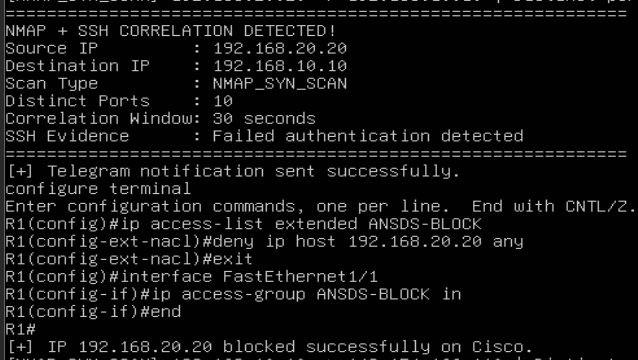
\includegraphics[width=0.95\textwidth]{figures/Fig-05-06_Nmap_SSH_Correlation.png}

    \caption{Corrélation entre un scan Nmap et une activité SSH suspecte}

    \label{fig:phase5-ssh-correlation}

\end{figure}

\subsection{Scan sans corrélation SSH}

Un deuxième scénario a été utilisé afin de vérifier qu'un scan Nmap seul ne déclenche pas automatiquement la même réponse qu'un événement corrélé avec une activité SSH.

\begin{figure}[H]

    \centering

    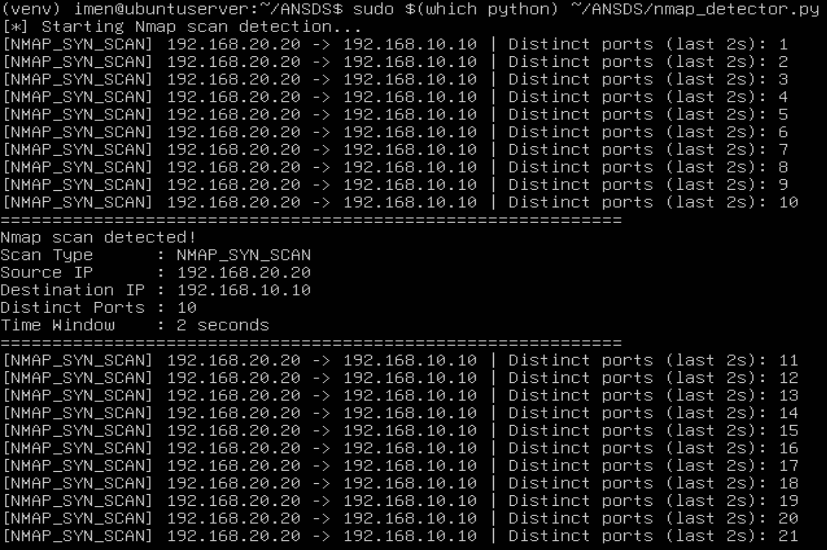
\includegraphics[width=0.95\textwidth]{figures/Fig-05-07_Nmap_Only_No_Correlation.png}

    \caption{Scan Nmap sans corrélation avec une activité SSH}

    \label{fig:phase5-no-correlation}

\end{figure}

Cette séparation permet de distinguer une activité de reconnaissance isolée d'un comportement combinant reconnaissance et tentative d'accès au service SSH.

\section{Notification de sécurité}

Lorsqu'une corrélation est confirmée, le système transmet un événement au module de notification Telegram.

Le module Telegram reste séparé du moteur de détection afin de conserver une architecture modulaire.

Le workflow est alors :

\begin{center}

Nmap Detection

$\downarrow$

SSH Correlation

$\downarrow$

Security Event

$\downarrow$

Telegram Notification

\end{center}

La notification permet à l'administrateur d'être informé de l'activité détectée avant ou pendant l'application de la mesure de protection réseau.

\section{Réponse automatique Cisco}

Après confirmation de l'événement de sécurité, le système peut déclencher le mécanisme de réponse automatique développé durant la phase précédente.

Le module Cisco utilise Netmiko afin d'établir une connexion SSH avec le routeur Cisco et d'appliquer dynamiquement une ACL \cite{netmiko_docs,cisco_ios}.

La règle de blocage utilisée est :

\begin{verbatim}

deny ip host \<SOURCE\_IP> any

\end{verbatim}

Cette approche permet de transformer automatiquement un événement de sécurité confirmé en mesure de protection réseau.

\subsection{Activation du blocage temporaire}

Contrairement à un blocage permanent, le mécanisme développé durant cette phase utilise une durée de blocage limitée.

Lorsqu'un événement est confirmé, le système applique le blocage puis programme automatiquement son expiration.

Le cycle de traitement est :

\begin{center}

Détection

$\downarrow$

Corrélation

$\downarrow$

Notification

$\downarrow$

Blocage Cisco

$\downarrow$

Expiration

$\downarrow$

Déblocage automatique

\end{center}

La capture suivante présente l'activation du blocage temporaire.

\begin{figure}[H]

    \centering

    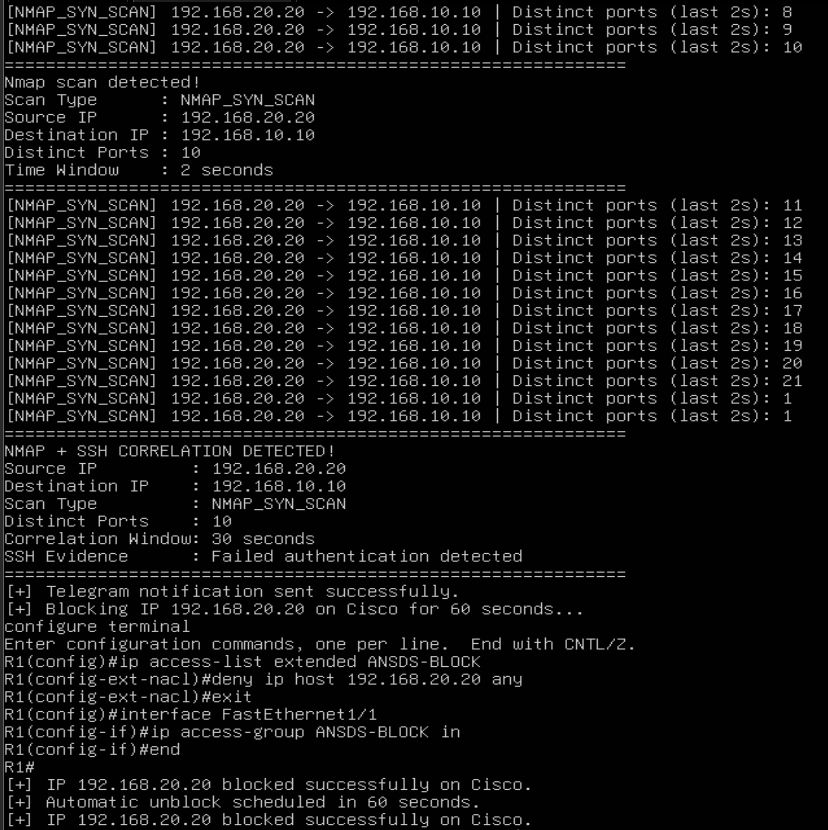
\includegraphics[width=0.95\textwidth]{figures/Fig-05-08_Temporary_Block_Activated.png}

    \caption{Activation du blocage temporaire}

    \label{fig:phase5-temporary-block}

\end{figure}

\subsection{Application de l'ACL Cisco}

Le module Cisco crée dynamiquement l'ACL destinée à bloquer l'adresse IP source.

L'application de cette règle est réalisée automatiquement à travers Netmiko \cite{netmiko_docs,cisco_ios}.

\begin{figure}[H]

    \centering

    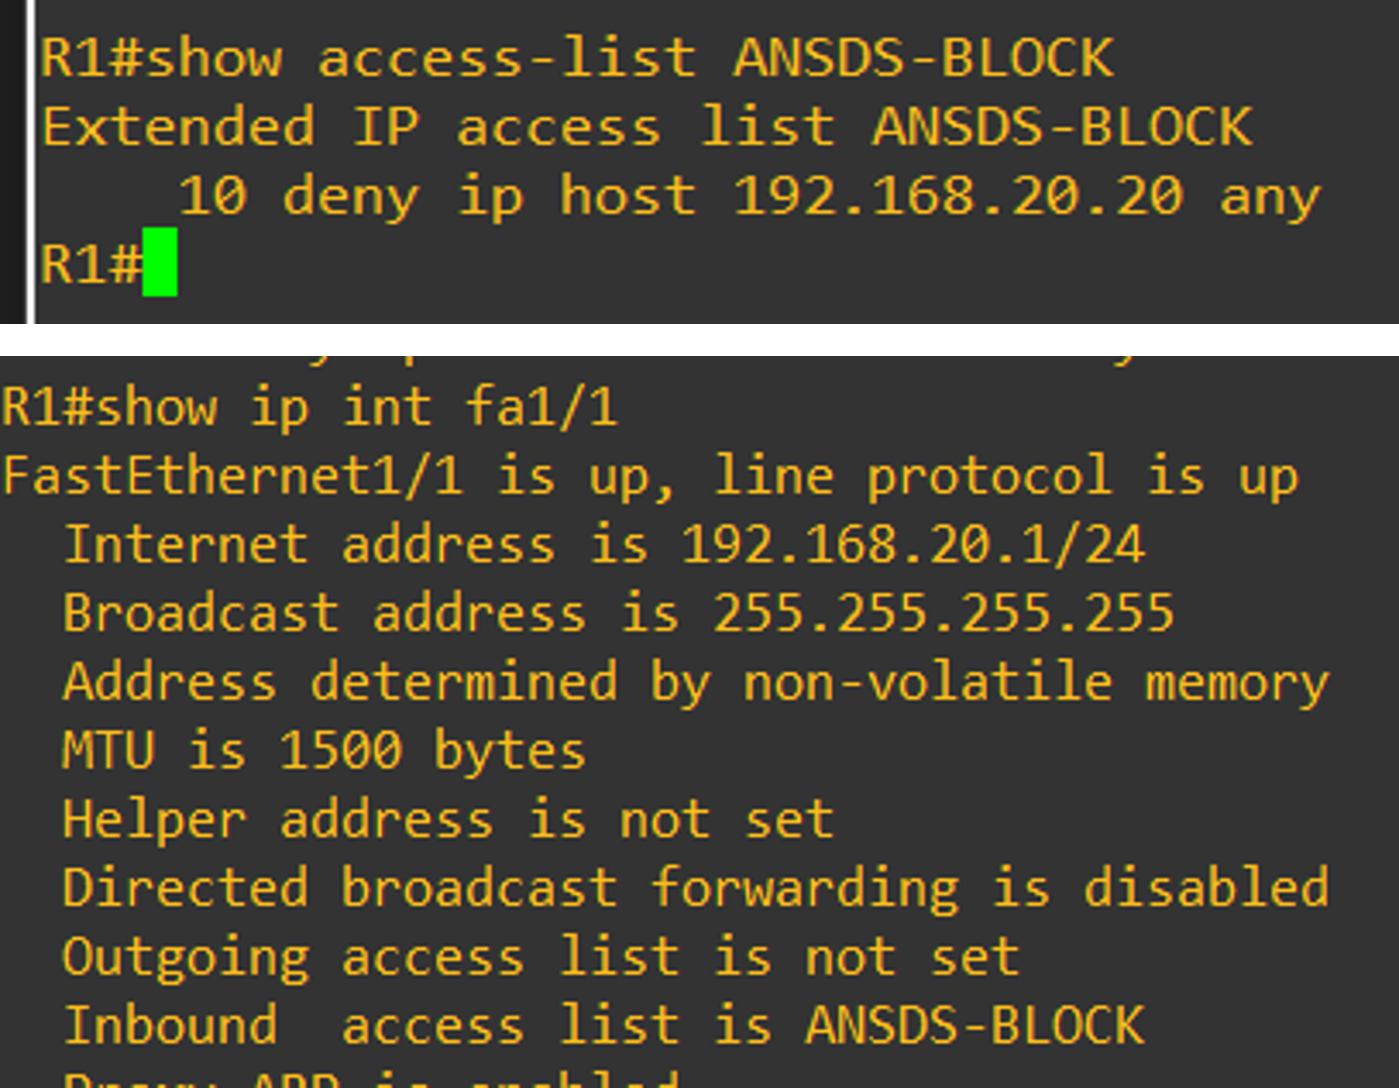
\includegraphics[width=0.95\textwidth]{figures/Fig-05-09_ACL_Block_Application.png}

    \caption{Application de l'ACL de blocage sur le routeur Cisco}

    \label{fig:phase5-acl-block}

\end{figure}

Cette étape confirme l'intégration entre le moteur de détection et l'infrastructure réseau.

\section{Journalisation des événements}

La Phase 5 introduit également un mécanisme de journalisation permettant de conserver une trace des événements de sécurité.

Le système journalise notamment :

\begin{itemize}

\item l'adresse IP source ;

\item l'adresse IP destination ;

\item le type de scan ;

\item le nombre de ports distincts ;

\item la fenêtre temporelle ;

\item la confirmation de la corrélation SSH ;

\item l'envoi de la notification Telegram ;

\item l'application du blocage Cisco ;

\item la durée du blocage ;

\item l'expiration du blocage ;

\item la suppression de l'ACL.

\end{itemize}

Le journal permet ainsi de reconstruire le cycle de traitement d'un événement de sécurité et facilite la validation du fonctionnement du système.

\section{Expiration automatique du blocage}

Le blocage appliqué par le système est temporaire.

À l'expiration de la durée configurée, le module Cisco supprime automatiquement la règle créée précédemment.

Cette fonctionnalité évite qu'une ACL temporaire reste active indéfiniment et permet au réseau de revenir automatiquement à son état initial.

Le cycle complet est donc :

\begin{center}

\textbf{**Detection**}

$\rightarrow$

\textbf{**Correlation**}

$\rightarrow$

\textbf{**Alert**}

$\rightarrow$

\textbf{**Block**}

$\rightarrow$

\textbf{**Expiration**}

$\rightarrow$

\textbf{**Unblock**}

\end{center}

\subsection{Suppression de l'ACL}

La suppression automatique de l'ACL est réalisée lorsque la durée de blocage arrive à expiration.

\begin{figure}[H]

    \centering

    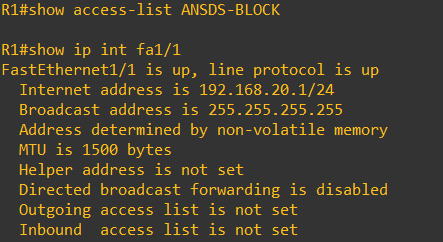
\includegraphics[width=0.95\textwidth]{figures/Fig-05-10_ACL_Removal.png}

    \caption{Suppression automatique de l'ACL après expiration du blocage}

    \label{fig:phase5-acl-removal}

\end{figure}

Cette fonctionnalité complète le cycle de vie du blocage temporaire.

\section{Architecture finale de la Phase 5}

À l'issue de cette phase, l'architecture du système peut être représentée par la chaîne suivante :

\begin{center}

Attacker

$\downarrow$

Scapy Packet Capture

$\downarrow$

Multi-Attack Detection

$\downarrow$

Nmap Scan Detection

$\downarrow$

SSH Correlation

$\downarrow$

Security Decision

$\downarrow$

Telegram Notification

$\downarrow$

Netmiko

$\downarrow$

Cisco Router

$\downarrow$

Dynamic ACL

$\downarrow$

Temporary Blocking

$\downarrow$

Automatic Unblocking

\end{center}

Cette architecture conserve la séparation des responsabilités entre les différents modules du projet.

Le moteur de détection est chargé de l'analyse du trafic, le module Telegram assure la notification, le module Cisco réalise la réponse réseau et le module de journalisation assure la traçabilité des événements.

\section{Validation expérimentale}

Une série d'expérimentations a été réalisée afin de valider progressivement les fonctionnalités introduites durant cette phase.

Les tests ont porté sur les éléments suivants :

\begin{itemize}

\item détection d'un Nmap SYN Scan ;

\item détection d'un Nmap FIN Scan ;

\item détection d'un Nmap NULL Scan ;

\item détection d'un Nmap Xmas Scan ;

\item observation d'un trafic légitime ;

\item corrélation entre une activité Nmap et une activité SSH ;

\item absence de corrélation lorsqu'aucune activité SSH correspondante n'est observée ;

\item transmission de la notification Telegram ;

\item activation du blocage temporaire ;

\item application de l'ACL Cisco ;

\item expiration du blocage ;

\item suppression automatique de l'ACL.

\end{itemize}

Les captures présentées dans ce chapitre constituent les éléments de preuve expérimentale associés à ces différents scénarios.

\section{Analyse des résultats}

Les expérimentations montrent que l'architecture ANSDS peut être étendue à plusieurs catégories d'événements réseau sans remettre en cause les composants développés durant les phases précédentes.

L'ajout de la détection Nmap permet au système d'observer une activité de reconnaissance en complément de la surveillance des tentatives SSH.

L'utilisation de plusieurs indicateurs améliore également la prise de décision. Une signature TCP isolée n'est pas considérée comme suffisante pour déclencher une réponse complète. Le comportement est analysé à travers les ports ciblés, la répétition des paquets, la fenêtre temporelle et, lorsque cela est pertinent, l'activité SSH associée.

La corrélation permet ainsi de distinguer une activité de reconnaissance isolée d'une séquence plus significative combinant scan réseau et tentative d'accès SSH.

L'intégration avec Telegram et Netmiko permet ensuite de conserver la chaîne automatisée développée lors des phases précédentes.

Enfin, le blocage temporaire et son expiration automatique permettent de gérer le cycle complet d'une mesure de protection réseau sans intervention manuelle.

\section{Journalisation et traçabilité}

Le système conserve désormais les événements importants du traitement dans le fichier de journalisation ANSDS.

Les événements permettent notamment de suivre :

\begin{verbatim}

NMAP\_DETECTED

SSH\_CORRELATION\_CONFIRMED

TELEGRAM\_ALERT\_SENT

IP\_BLOCKED

TEMPORARY\_BLOCK\_SCHEDULED

TEMPORARY\_BLOCK\_EXPIRED

IP\_UNBLOCKED

\end{verbatim}

Cette journalisation fournit une trace chronologique des décisions prises par le système et permet de vérifier que les différents composants ont correctement exécuté leur rôle.

\section{Conclusion}

Cette phase a permis d'étendre le système ANSDS au-delà de la simple détection des tentatives SSH.

Un mécanisme de détection des scans Nmap a été intégré afin d'identifier plusieurs comportements de reconnaissance réseau à partir des signatures TCP observées avec Scapy \cite{scapy_docs}.

Les quatre types de scans étudiés sont les scans SYN, FIN, NULL et Xmas.

La détection repose sur l'analyse comportementale de plusieurs paquets et de plusieurs ports plutôt que sur l'observation d'un paquet isolé.

La Phase 5 introduit également une logique de corrélation avec l'activité SSH. Cette approche permet de renforcer la décision de sécurité en combinant les informations provenant de plusieurs indicateurs.

Lorsque l'événement est confirmé, le système peut transmettre automatiquement une notification Telegram puis appliquer une ACL dynamique sur le routeur Cisco à l'aide de Netmiko \cite{netmiko_docs,cisco_ios}.

Le blocage est temporaire et son expiration entraîne automatiquement la suppression de l'ACL.

Enfin, la journalisation fournit une traçabilité des différentes étapes du traitement.

La chaîne obtenue peut être résumée ainsi :

\begin{center}

\textbf{**Network Reconnaissance**}

$\rightarrow$

\textbf{**Nmap Detection**}

$\rightarrow$

\textbf{**SSH Correlation**}

$\rightarrow$

\textbf{**Security Alert**}

$\rightarrow$

\textbf{**Telegram**}

$\rightarrow$

\textbf{**Cisco ACL**}

$\rightarrow$

\textbf{**Temporary Block**}

$\rightarrow$

\textbf{**Automatic Unblock**}

\end{center}

Cette évolution constitue une étape supplémentaire vers un système ANSDS capable de détecter et de traiter automatiquement plusieurs comportements malveillants au niveau réseau.